\documentclass[a4paper,onecolumn]{article}
\usepackage{amsmath, amsthm, graphicx, amssymb, wrapfig, fullpage, subfigure, array}
\usepackage{tikz}
\usetikzlibrary{positioning,shadows,arrows}
\usepackage[font=sl, labelfont={sf}, margin=1cm]{caption}
\DeclareMathOperator{\e}{e}
\newtheorem{mydef}{Definition}
\theoremstyle{remark}
\newtheorem{remarker}{Remark}

\begin{document}
\setcounter{page}{1}

\title{Implement An Unsupervised Learning Machine \\ and Corrupted Data Reconstruction}
\author{Han Chen}
\maketitle

\section{Results}
\begin{itemize}
    \item First column: original image. 
    \item Second column: corrupt image by covering the top half.
    \item Third column: image inferred from the corrupted image.
\end{itemize}
\begin{center}
    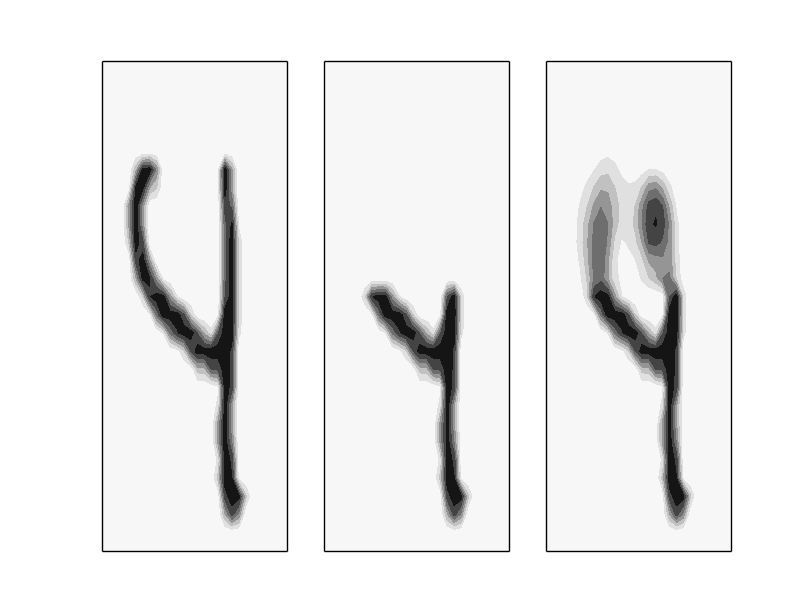
\includegraphics[width=9cm,height=2.5cm]{png/recon1.png}\\
    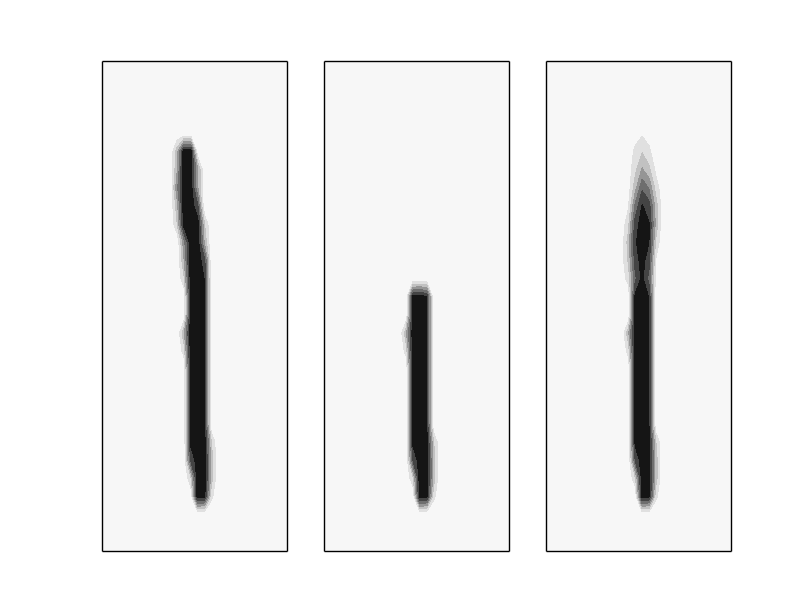
\includegraphics[width=9cm,height=2.5cm]{png/recon2.png}\\
    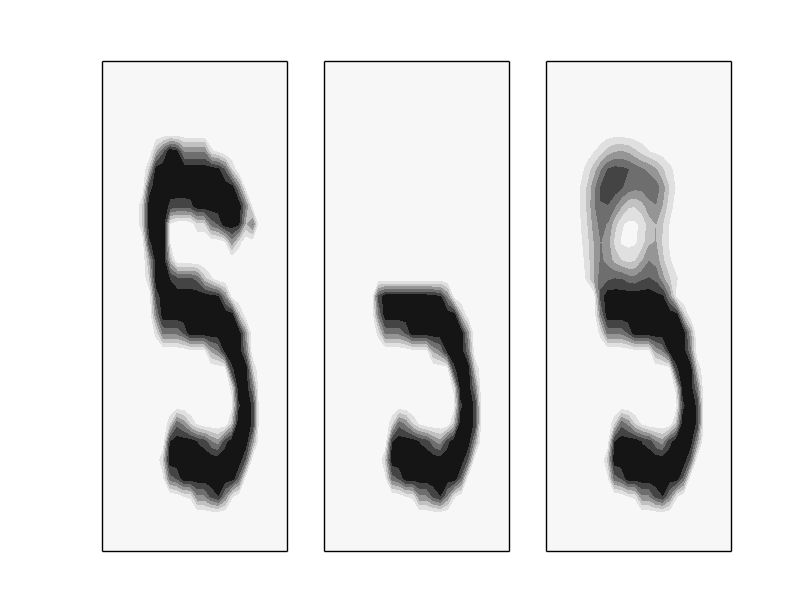
\includegraphics[width=9cm,height=2.5cm]{png/recon3.png}\\
    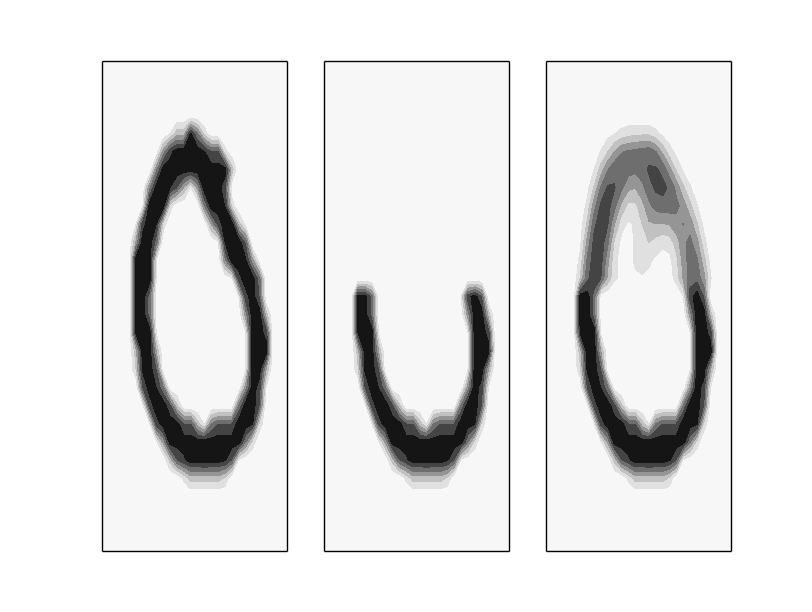
\includegraphics[width=9cm,height=2.5cm]{png/recon4.png}\\
    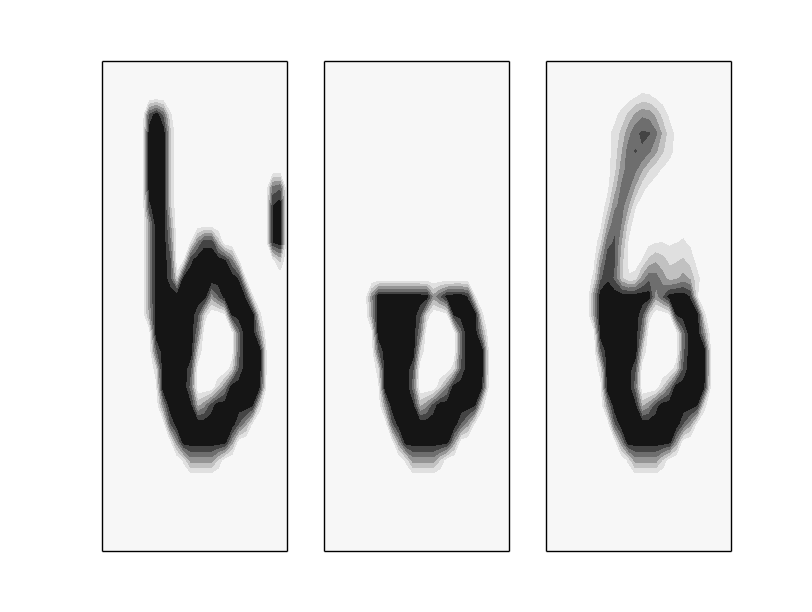
\includegraphics[width=9cm,height=2.5cm]{png/recon5.png}\\
    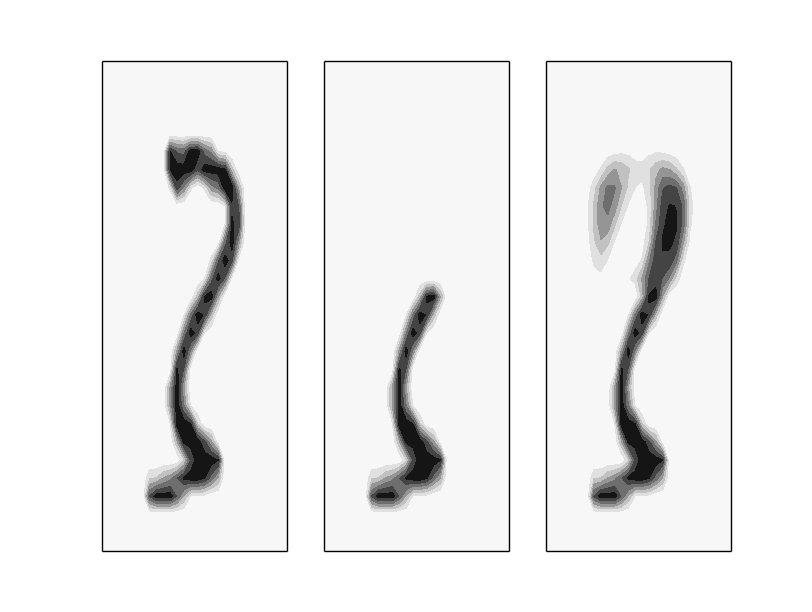
\includegraphics[width=9cm,height=2.5cm]{png/recon6.png}
\end{center}

\section{Restricted Boltzmann Machine}
\begin{center}
        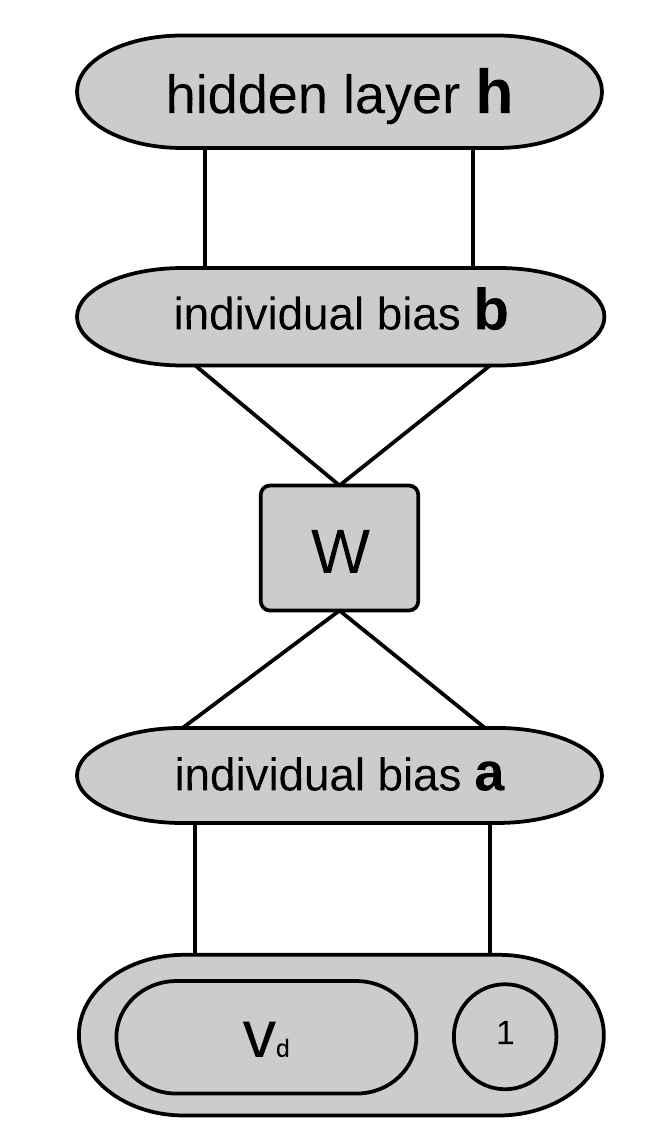
\includegraphics[width=4cm]{RBM.png}
\end{center}
The visible and hidden variables are conditional Bernoulli
\begin{equation}\begin{split}
    P(v_i=1 \big| h) &= \sigma (a_i + W_{i,\cdot}\cdot h)\\
    P(h_j=1 \big| v) &= \sigma (b_j + W_{\cdot,j}\cdot v)
\end{split}\,,\end{equation}
where 
\begin{equation}
    \sigma(x) = \frac{1}{1+e^{-x}}\,.
\end{equation}
Gradient of data log-likelihood
\begin{equation}\begin{split}
    \frac{\partial \log p(v)}{\partial W_{i,j}} &= 
    <v_i h_j>_{\textrm{data}} - <v_i h_j>_{\textrm{model}}\\
    \frac{\partial \log p(v)}{\partial a_i} &=
    <v_i>_{\textrm{data}} - <v_i>_{\textrm{model}}\\
    \frac{\partial \log p(v)}{\partial b_j} &=
    <h_j>_{\textrm{data}} - <h_j>_{\textrm{model}}
\end{split}
\label{gradlike}
\end{equation}

\subsection{Sampling by Contrastive-Divergence}
Let $N$ be the cardinality of the training data. The integrals in \eqref{gradlike} can
be approximated by
\begin{equation}\begin{split}
    <v_i h_j>_{\textrm{data}} &\approx \frac{1}{N} \sum_{n=1}^N 
    v_i^{(n)} h_j^{(n)}\\
    <v_i>_{\textrm{data}} &\approx \frac{1}{N} \sum_{n=1}^N v_i^{(n)}\\
    <h_j>_{\textrm{data}} &\approx \frac{1}{N} \sum_{n=1}^N
    \sigma\big(b_j + W_{\cdot,j} v^{(n)}\big)
\end{split}\,,\quad
h_j^{(n)} \sim P(h_j=1\big| v^{(n)})
\label{data integral}
\end{equation}
and
\begin{equation}\begin{split}
    <v_i h_j>_{\textrm{model}} &\approx
    \frac{1}{N} \sum_{n=1}^N  \sigma \big(a_i + W_{i,\cdot}\cdot h^{(n)}\big) \, h_j^{(n)}\\
    <v_i>_{\textrm{model}} &\approx
    \frac{1}{N}\sum_{n=1}^N \sigma \big(a_i + W_{i,\cdot}\cdot h^{(n)}\big) \\
    <h_j>_{\textrm{model}} &\approx \frac{1}{N}\sum_{n=1}^N 
    \sigma(b_j + W_{\cdot, j} \cdot \hat{v}^{(n)})
\end{split}\,,\quad
\begin{split}
h_j^{(n)} &\sim P(h_j=1\big| v^{(n)})\\
\hat{v}^{(n)} &\sim P(\hat{v}_i=1\big| h^{(n)})
\end{split}
\label{model integral}
\end{equation}
\eqref{data integral} and \eqref{model integral} can be expressed by the graphical model 
\begin{center}
        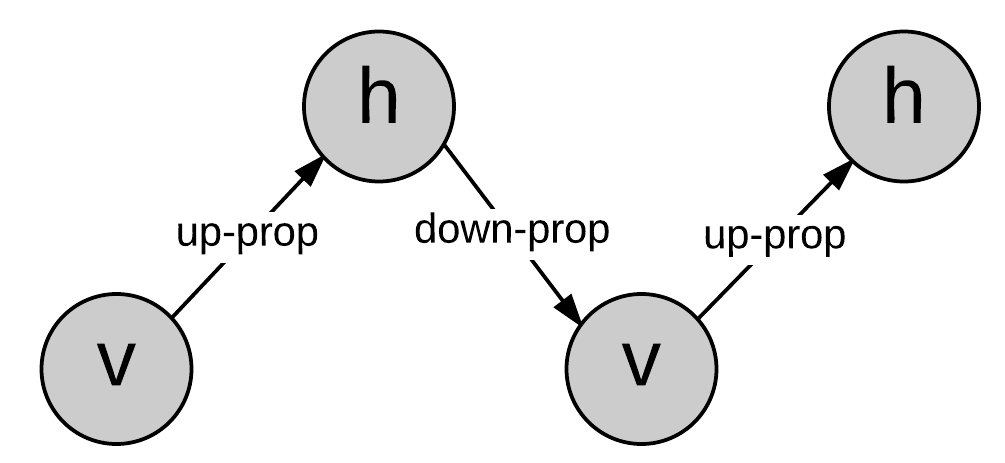
\includegraphics[width=6cm]{CD1.png}
\end{center}
In the implementation, the up-propogation and down-propogation methods produce both the 
probability and a binary sampling.

\subsection{Stochastic Gradient Descent}
Given a learning rate,
\eqref{data integral} and \eqref{model integral} drives the maximization of data log-likelihood
by stochastic gradient descent according to \eqref{gradlike}.

\subsection{Regularization}
An L-1 regularizer for the weights is implemented into the log-likelihood, which modifies 
\eqref{gradlike} to
\begin{equation}\begin{split}
    \frac{\partial \log p(v)}{\partial W_{i,j}} &= 
    <v_i h_j>_{\textrm{data}} - <v_i h_j>_{\textrm{model}} - \lambda \delta_{W_{i,j}}\\
    \frac{\partial \log p(v)}{\partial a_i} &=
    <v_i>_{\textrm{data}} - <v_i>_{\textrm{model}}\\
    \frac{\partial \log p(v)}{\partial b_j} &=
    <h_j>_{\textrm{data}} - <h_j>_{\textrm{model}}
\end{split}\,,
\label{gradlike L1}
\end{equation}
where 
\begin{equation}
    \delta_x = \left\{\begin{split}
        1&\,,\quad x>0\\
        0&\,,\quad x=0\\
        -1&\,, \quad x<0\\
    \end{split}\right.
\end{equation}
and
$\lambda>0$ is a small number.

\subsection{Termination Condition}
The training terminates when the free energy 
of the validation dataset exceeds the free energy of the training data by a certain amount.
The free energy is defined by
\begin{equation}
    \mathcal{F}(x) = - a\cdot v - \sum_{j=1}^H 
    \log \Big(
    1 + \exp\left(b_j + W_{\cdot, j} \cdot v\right)
    \Big)
\end{equation}

\section{Stacked Restricted Boltzmann Machine}
\begin{center}
    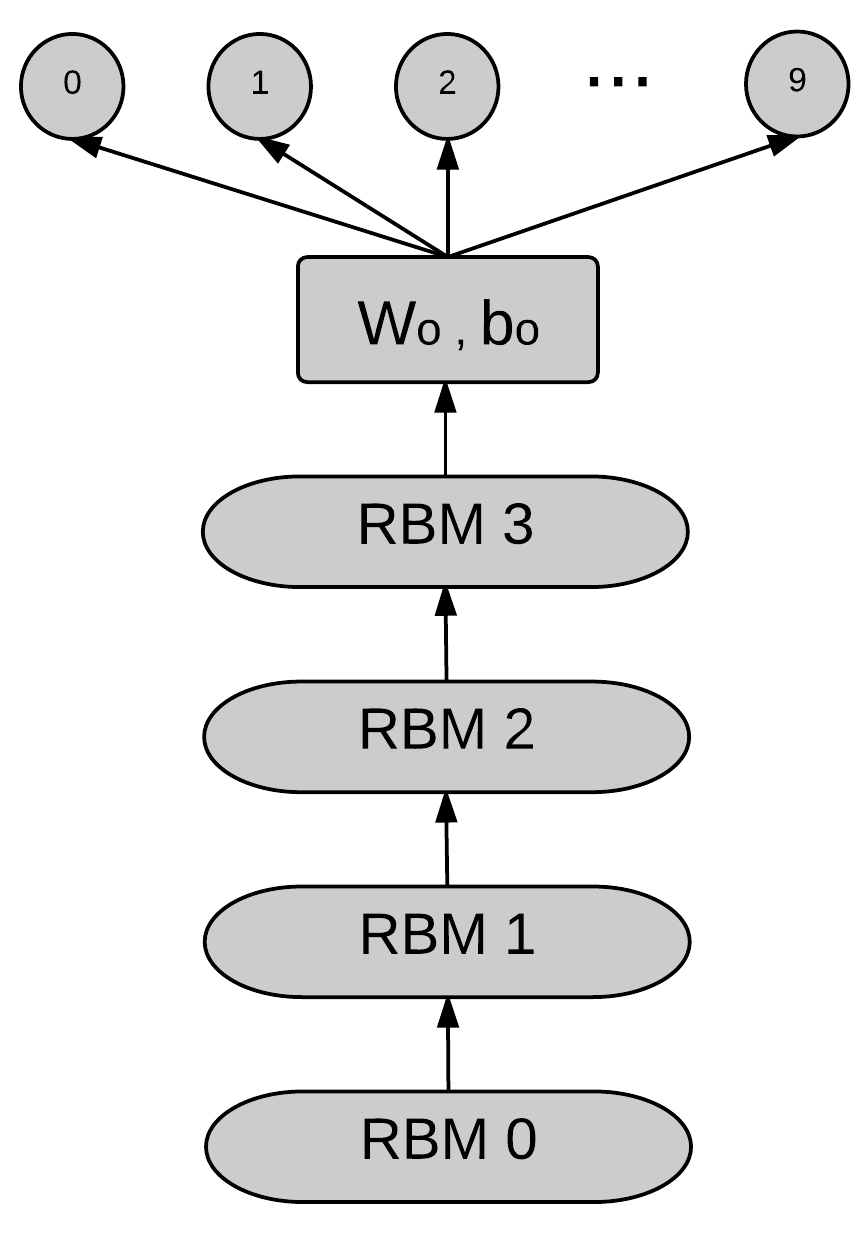
\includegraphics[width=4cm]{stacked.png}
\end{center}
\subsection{Fine Tuning}
After the tuning of each RBM, the RBMs are stacked into a deep neural network. 
The neural network is implemented using automatic
differentiation whose weights and biases are initialized by the unsupervised trained results.
The network is tuned by back propogation, where gradients are computed by automatic differentiation.

\section{Trained RBM Weights}
\begin{center}
    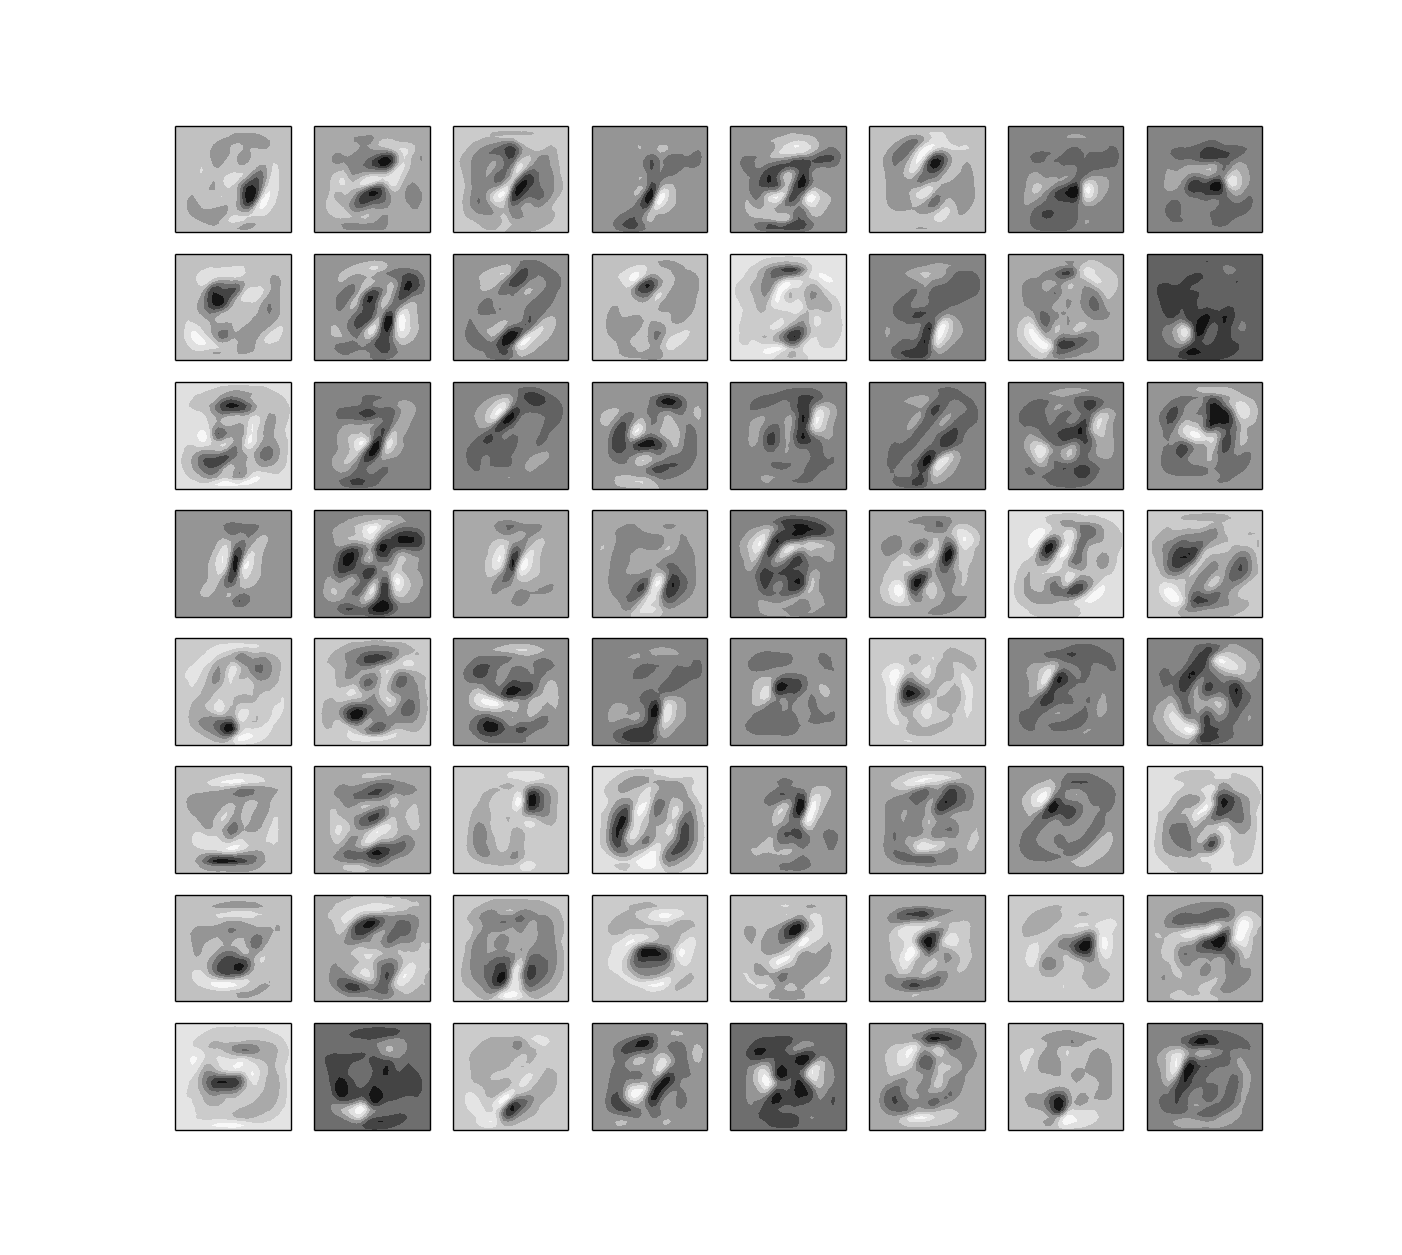
\includegraphics[width=12cm]{png/weight.png}
\end{center}

\section{Gibbs Sampling Transition}
\begin{center}
    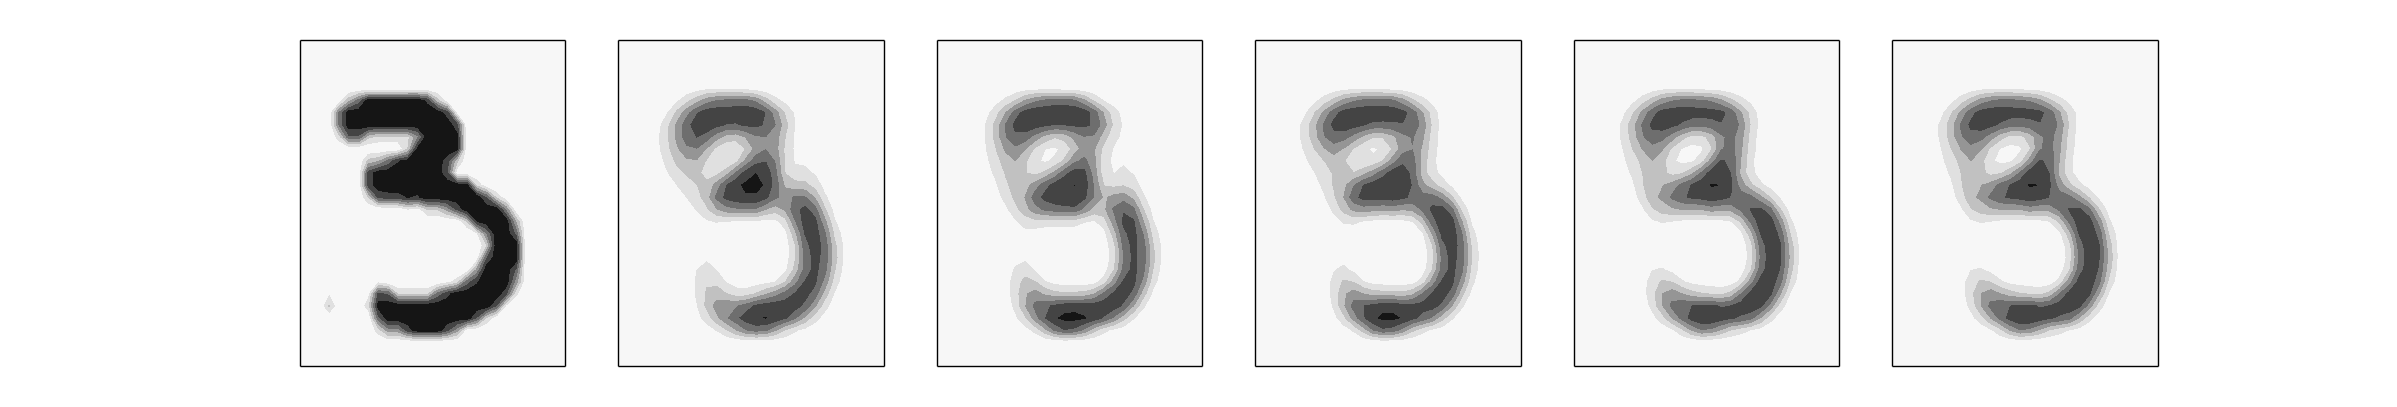
\includegraphics[width=12cm]{png/1.png}\\
    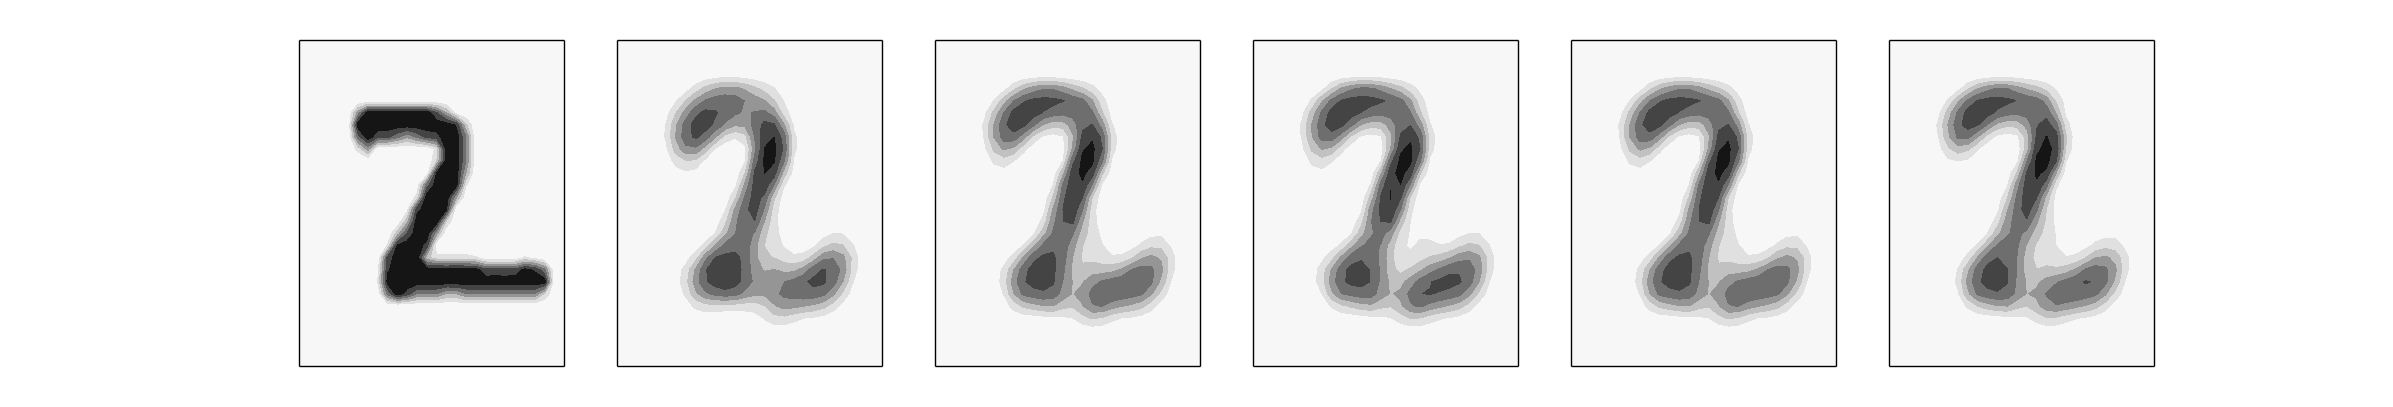
\includegraphics[width=12cm]{png/2.png}\\
    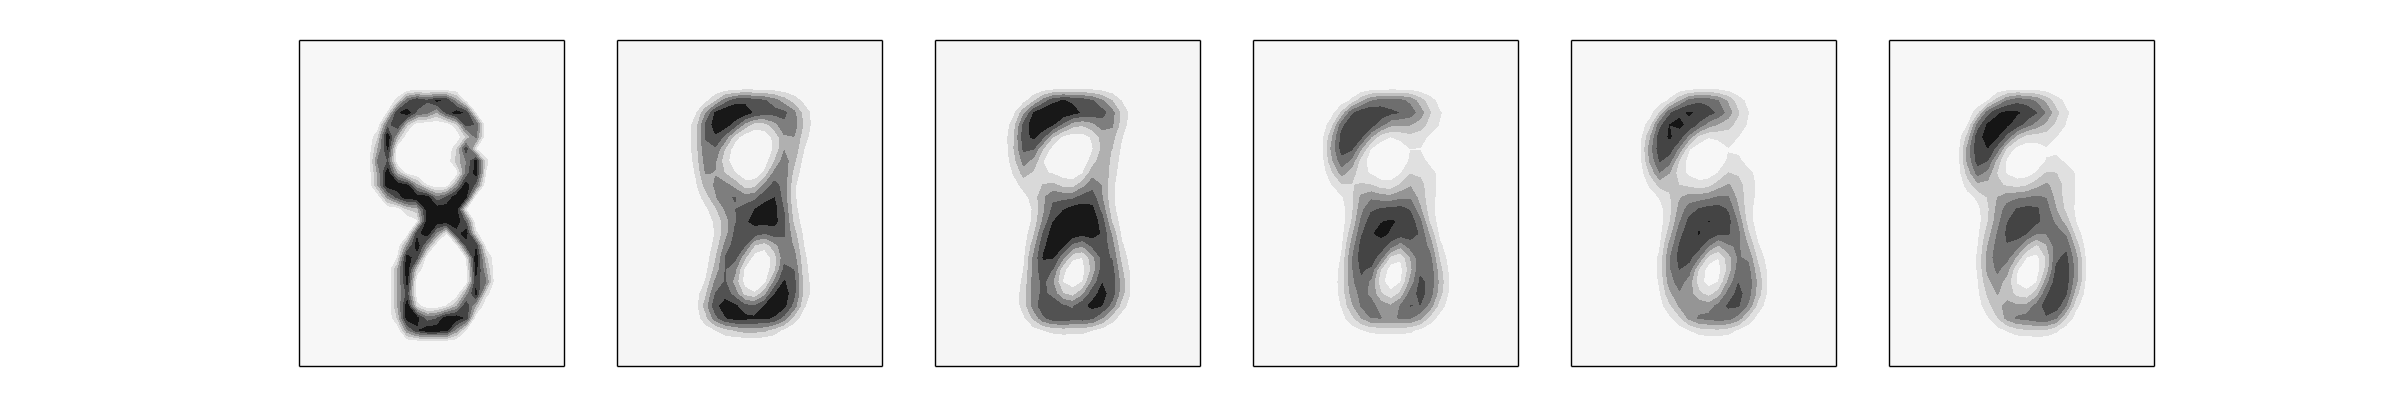
\includegraphics[width=12cm]{png/3.png}\\
    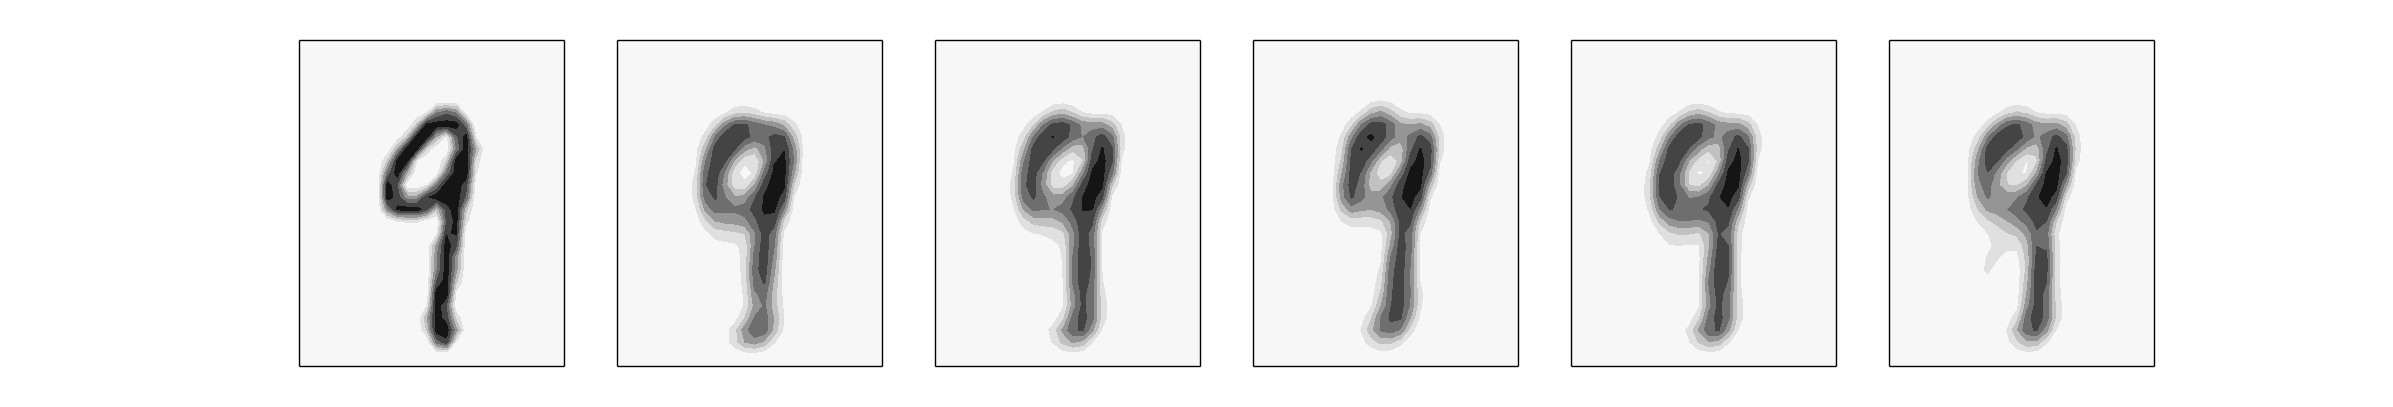
\includegraphics[width=12cm]{png/4.png}\\
    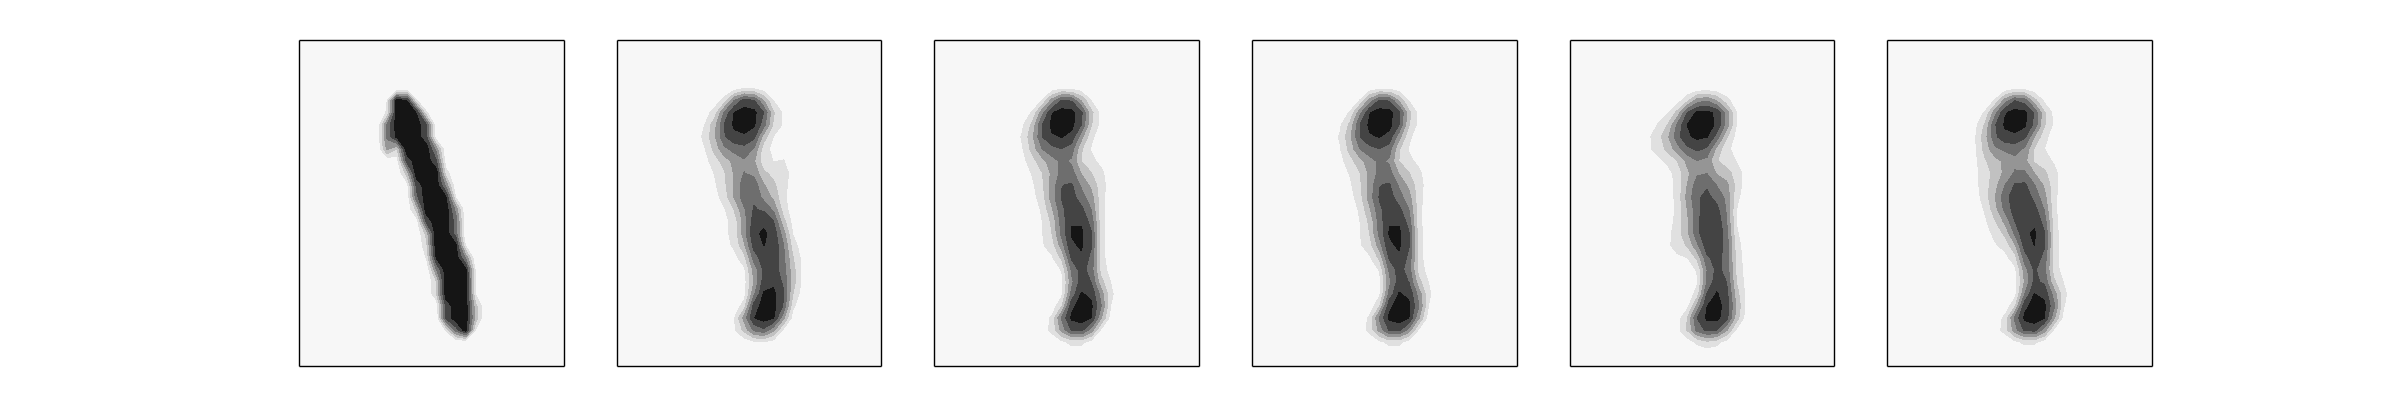
\includegraphics[width=12cm]{png/5.png}\\
    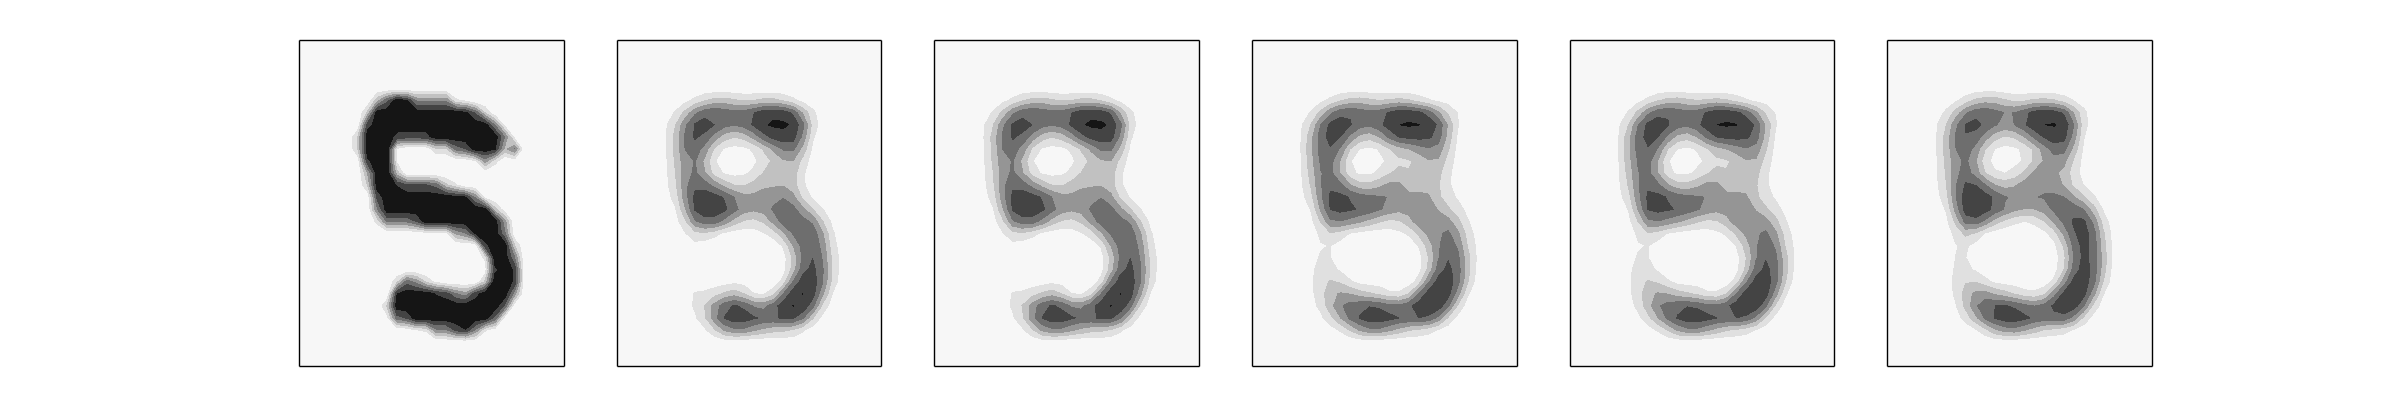
\includegraphics[width=12cm]{png/6.png}
\end{center}

\end{document}








